\documentclass[12pt]{article}

\usepackage[spanish]{babel}
\usepackage[utf8]{inputenc}
\usepackage{graphicx}
\usepackage{geometry}
\usepackage{xcolor}
\usepackage{fancyhdr}
\usepackage{lastpage}
\usepackage{pdfpages}
\usepackage{listings}

\geometry{top=25mm,left=15mm,right=15mm,a4paper}

\pagestyle{fancy}
\fancyhf{}
\lhead{Seminario de Ciencias de la Computación A}
\cfoot{Página \thepage\ de \pageref{LastPage}}

\graphicspath{./}

\begin{document}
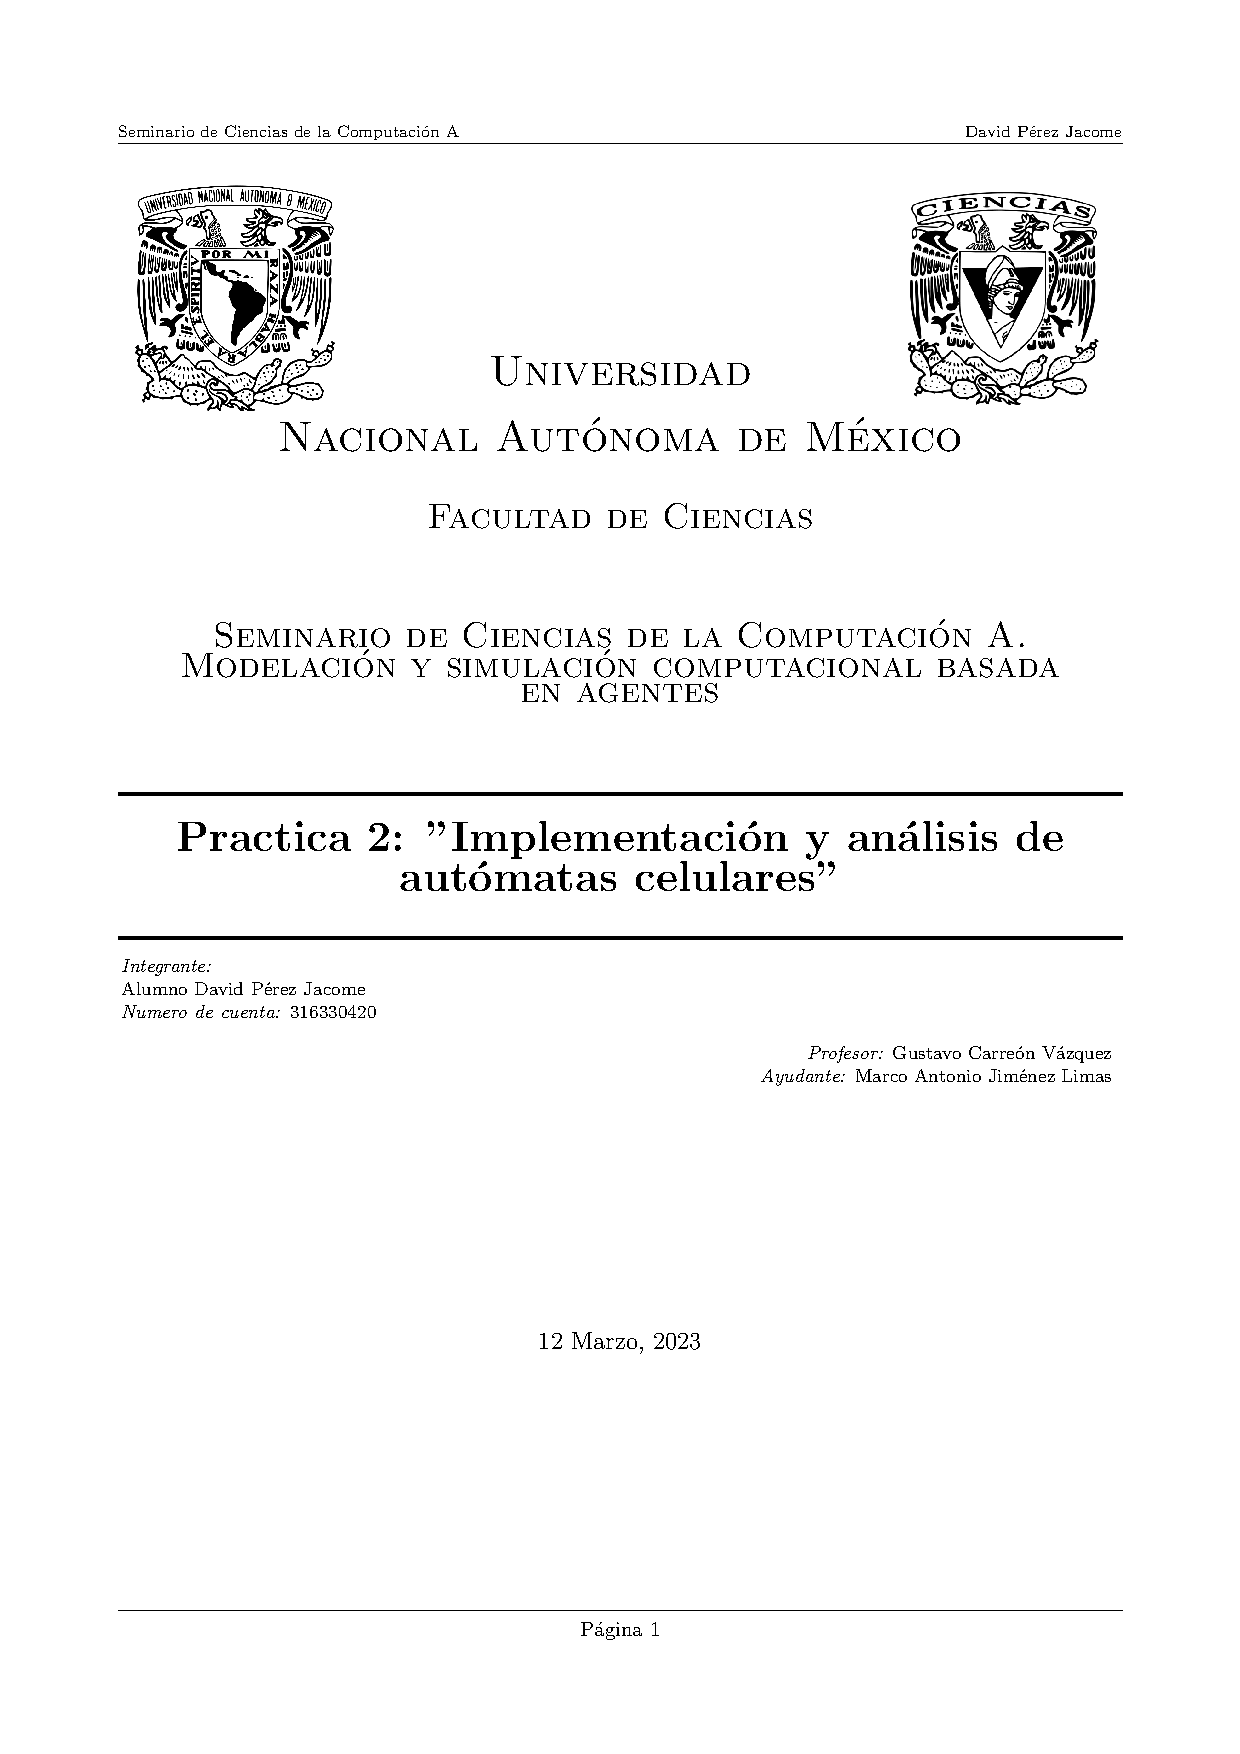
\includepdf{Portada.pdf}
{\color{red} \section*{Practica 3: Modelación de una dinámica de epidemias
con MBA.}}
\vspace{2em}

{\color{blue} \subsection*{Parte 1. Modelo basado en agentes SIR con distanciamiento social.}}
\vspace{1em}

Cada vez son más utilizados los modelos y simulaciones computacionales para recrear escenarios de los fenómenos y tomar mejores
decisiones. La actual pandemia que estamos viviendo requiere de su estudio y análisis desde distintos enfoques. Con la modelación
basada en agentes se puede entender la estrategia de distanciamiento social, su efectividad e impacto en la disminución de casos a lo
largo del tiempo. En el árticulo de Harry Stevens se propone un modelo para explicar los beneficios del distanciamiento social en una dinámica de contagio.\\

\textbf{Implementación del modelo en NetLogo}\\

El sistema se compone de una reticula de $n$ x $n$ donde $n=100$. Se colocan $k$ agentes (personas) distribuidos aleatoriamente sobre el sistema.\\

Estas personas pueden estar en uno de tres posibles estados: \textbf{sano, enfermo o recuperado}. Asigne un color para visualizar, por ejemplo, \textbf{sano=azul}, \textbf{enfermo=rojo} y \textbf{recuperado=verde}.
Las personas son caminadores aleatorios con un rango de visión determinado.\\

\textbf{Reglas:}\\

\begin{enumerate}
    \item \textbf{Contagio:} Si una persona sana tiene una persona enferma en su vecindad de Moore entonces se contagia con cierta probabilidad y cambia su estado a enfermo. Una persona
    enferma no puede contagiar nuevamente a una persona recuperada.
    \item \textbf{Recuperación:} Una persona enferma se recupera después de $k$ tiempos y cambia su estado a recuperado.
    \item \textbf{Movimiento:} Las personas son caminantes aleatorios con un rango de visión determinado (por ejemplo $-60$ y $60$ grados).
    \item \textbf{Distanciamiento social:} El distanciamiento social es una estrategia para mitigar los efectos de contagio en una pandemia. Las personas se exponen lo menos posible en lugares concurridos. En el modelo, las personas que
    apliquen distanciamiento social no se moverán como en el artículo de Harry Stevens.
\end{enumerate}

\textbf{Parámetros globales:}\\

Los parametros globales determinan el comportamiento del sistema y tiene un rango para establecer los valores:\\

\begin{enumerate}
    \item Densidad de la población \textbf{(POB)} de $10$ a $100\%$ en función del número de patches en el mundo.
    \item Apertura de visión del agente \textbf{(WIG)} de $10$° a $360$°.
    \item Probabilidad de contagio \textbf{(PC)}, se establece en el intervalo $0$ a $1$. Los casos extremos son: si es $0$ la persona infectada no puede transmitir la enfermedad; si es $1$ la persona infectada
    transmite la infección inmediatamente.
    \item Tiempo de la enfermedad \textbf{(TE)} de $10$ a $100$ tiempos o tiks.
    \item Distanciamiento social\textbf{(DS)} de $10$ a $100\%$ de la población, es el porcentaje de la población que hace distanciamiento social.
\end{enumerate}

{\color{blue} \subsubsection*{Experientos.}}
\vspace{1em}

\begin{enumerate}
    \item Como escenario inicial, establezca un tamaño de población $POB=30\%$, distanciamiento social, $DS=0\%$, Tiempo de enfermedad $TE=10$ ticks, Apertura de visión, $WIG=60$° y $PC=50\%$. En el inicio establezca algunos enfermos par iniciar el contagio.
    Grafique personas enfermas y recuperadas vs  el tiempo.\\
    \begin{enumerate}
    \item \textbf{¿Cómo son las curvas?}\\
    \textbf{Respuesta:} Se puede ver en la imagen del modelo, que las curvas con un tanto cerradas, y en un tiempo $t$ cambia drasticamente su comportamiento.\\
    \textbf{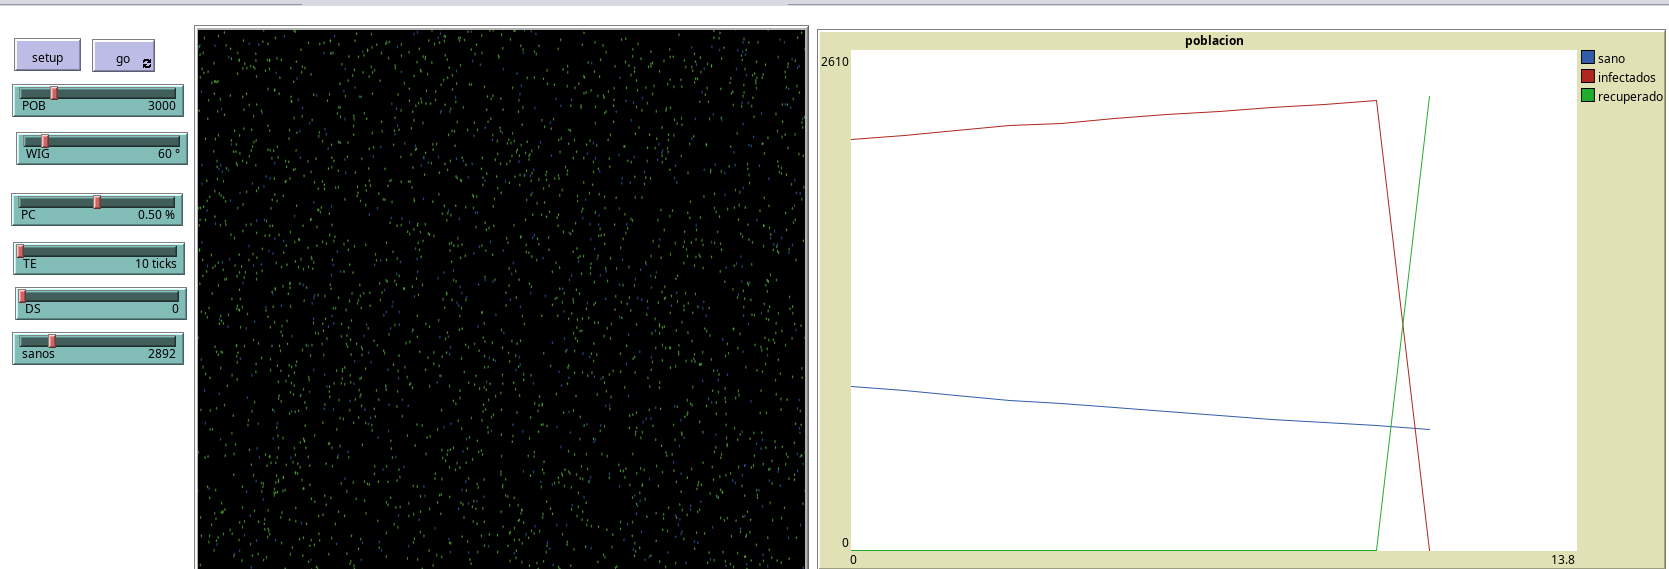
\includegraphics[scale = 0.30]{images/p1.png}}
    \item \textbf{¿En algún momento crece exponencialmente?}
    \textbf{Respuesta:} Si, llega un momento donde la cantidad de agentes sanos o curados crece de manera exponencial, mientras que los enfermos decrecen.
    \end{enumerate}

    \textbf{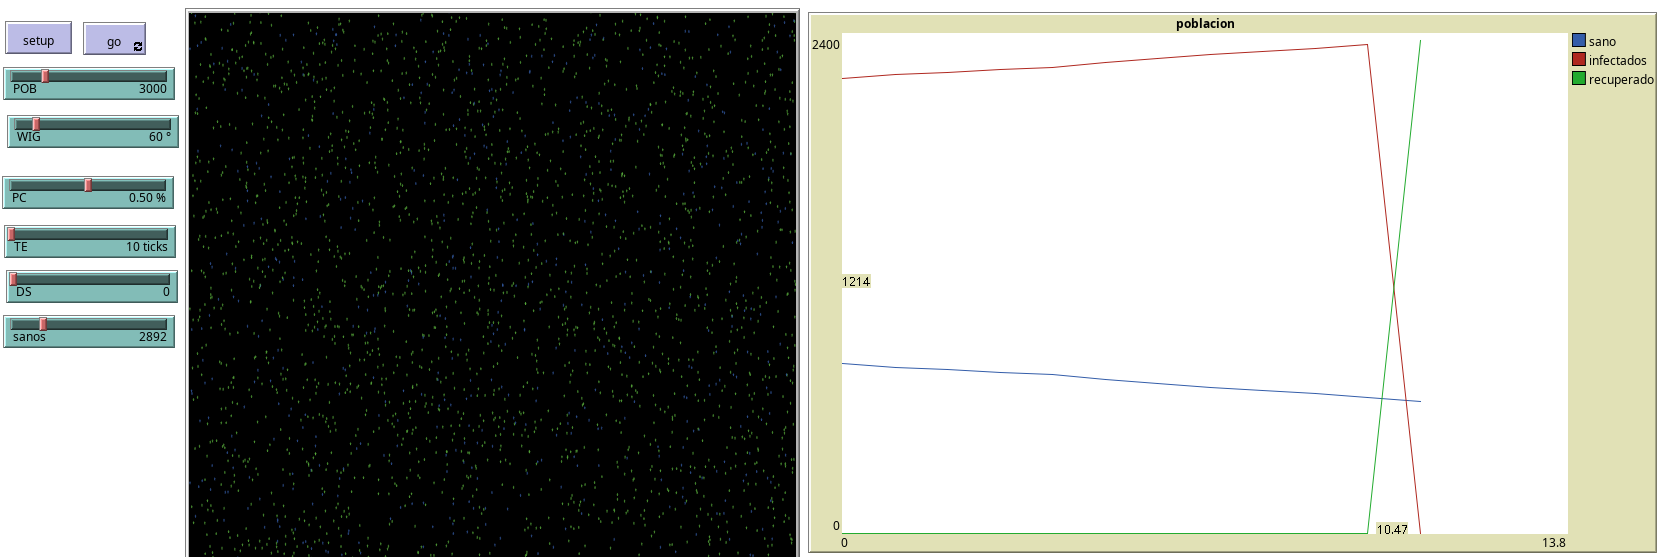
\includegraphics[scale = 0.30]{images/p1-1.png}}\\
    podemos observar que al igual que en la primer captura esta es otra ejecución del modelo, en el que si podemos ver la cantidad de sanos va en declive,
    mienstras que los enfermos en un punto preciso del experimento decrecen de manera exponencial, mientras que por otro lado, los agentes sanos van en crecimiento.


    \item Realice variaciones de los valores de los parámetros para replicar de manera cualitativa las curvas caracteristicas del modelo SIR con la unica restricción de mantener $DS=0\%$.
    Reporte los parámetros y la grafica con las curvas.\\

    \textbf{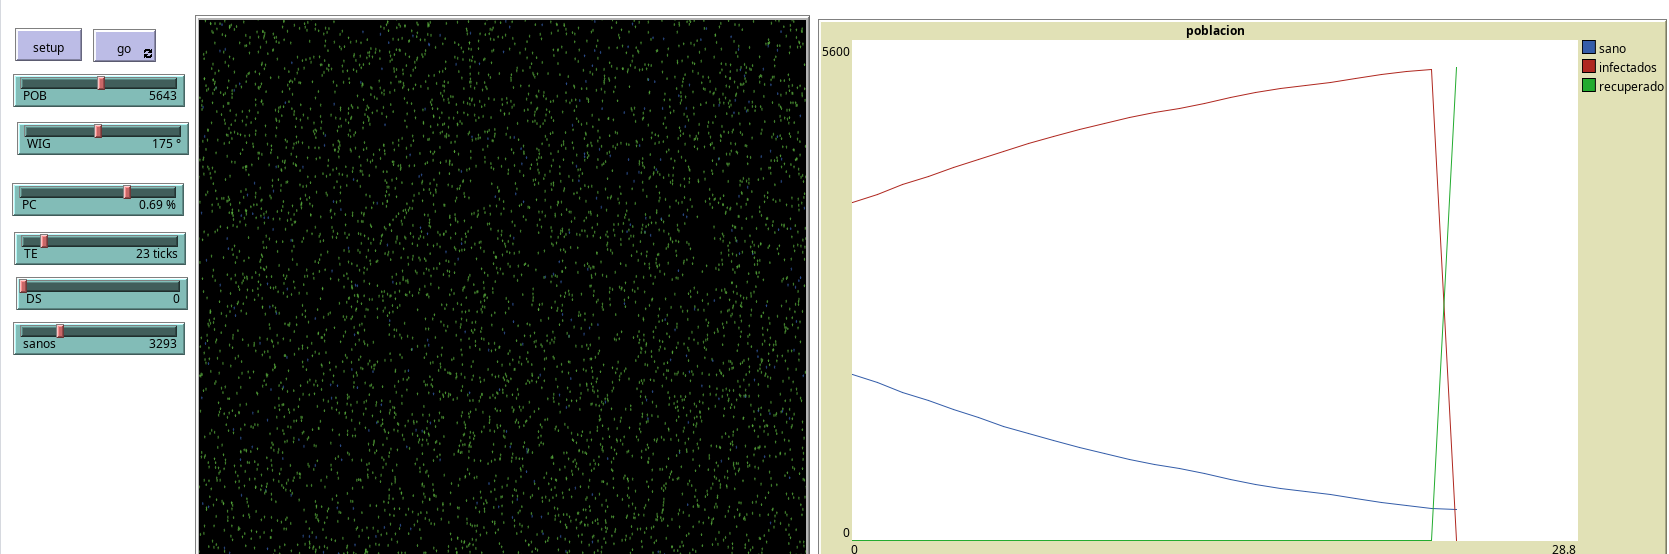
\includegraphics[scale = 0.30]{images/2-0.png}}\\
    en esta ocaciones tenemos $POB=50\%$, $WIG=175$°, $PC=69\%$, $TE=23ticks$, $sanos=30\%$.\\

    \textbf{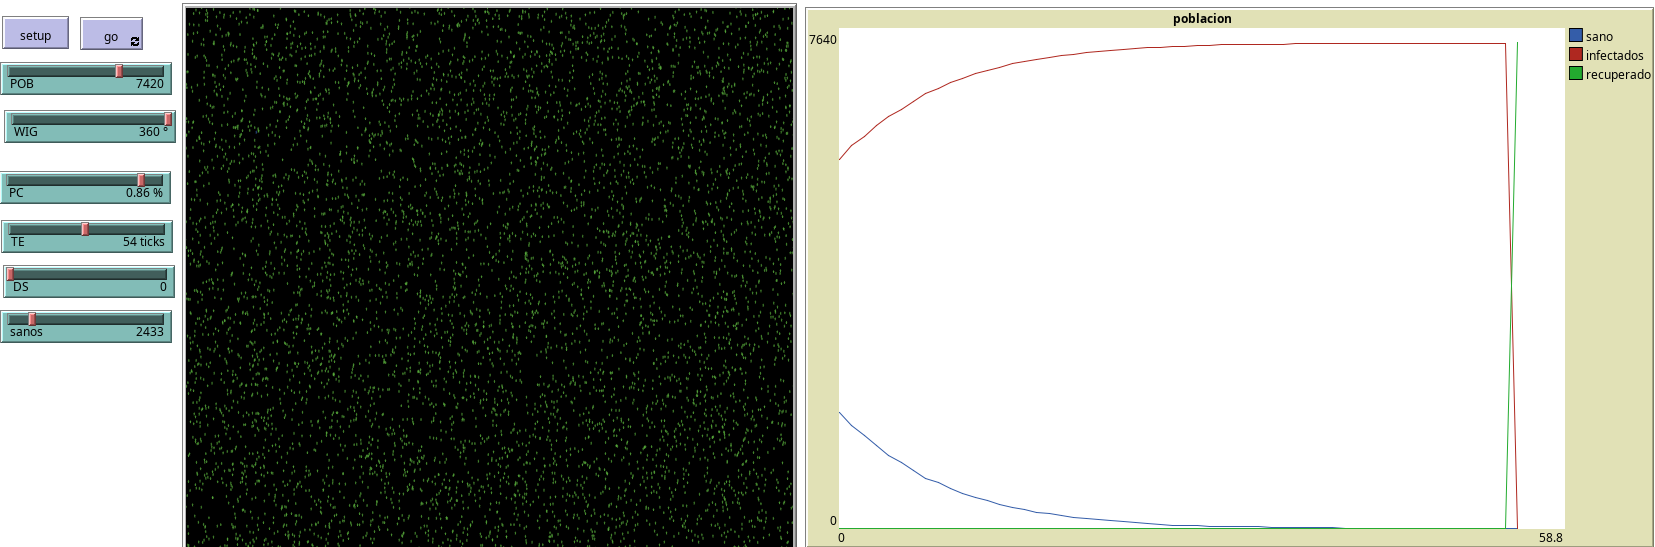
\includegraphics[scale = 0.30]{images/2-1.png}}\\
    en esta ocaciones tenemos $POB=70\%$, $WIG=360$°, $PC=86\%$, $TE=50ticks$, $sanos=10\%$.\\

    \textbf{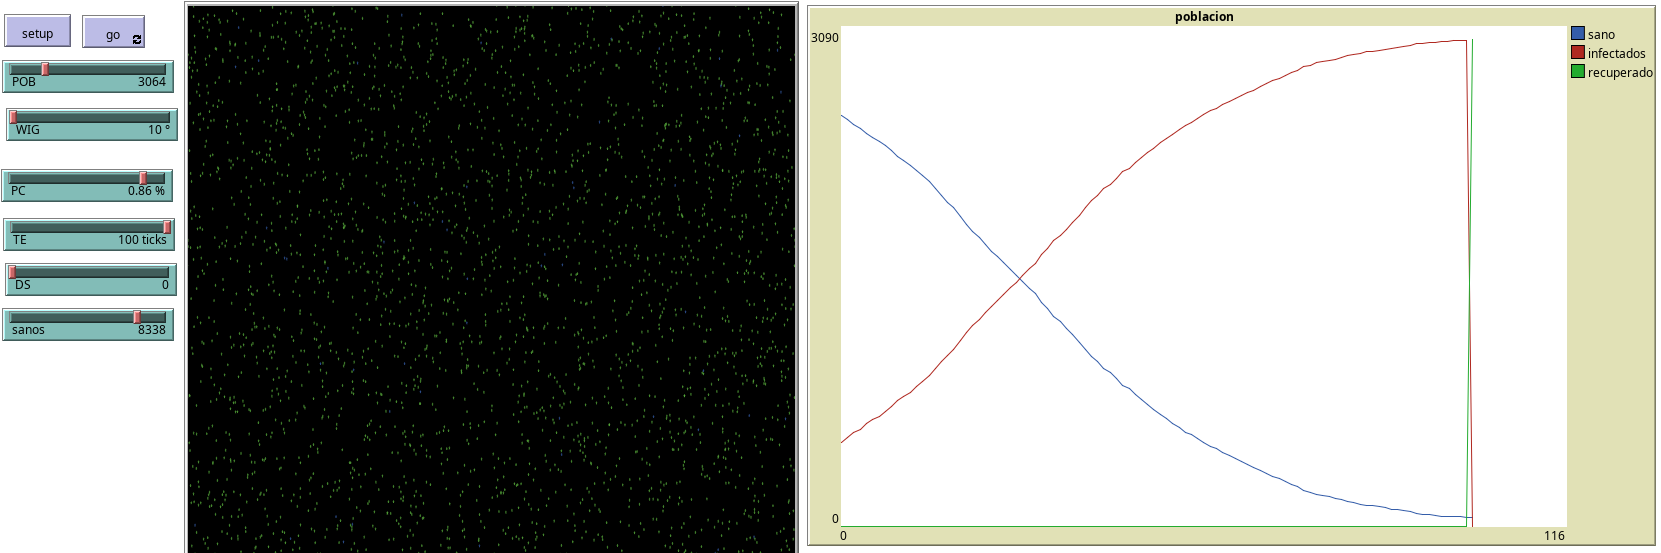
\includegraphics[scale = 0.30]{images/2-2.png}}\\
    en esta ocaciones tenemos $POB=30\%$, $WIG=10$°, $PC=90\%$, $TE=100ticks$, $sanos=80\%$.\\
    
    
    
    \item Con los parametros del ejercicio 2, establezca distanciamiento social $DS=25\%$.
    \begin{enumerate}
        \item \textbf{¿Cómo cambio la grafica de enfermos, infectados y recuperados?}.
        Pude darme cuenta que cambiaba al menos en el caso donde teniamos mas poblacion y un distanciamiento mayor se formaba mas la curva que en el otro caso donde cada una crecia en su respectivo Tiempo
        aunque claro que al llegar a los ticks correspondientes la simulación acababa y  crecia el número de curados.
        \item \textbf{Ahora $DS=50\%$ y $DS=75\%$.}\\
        Con $DS=50\%$:\\
        
        \textbf{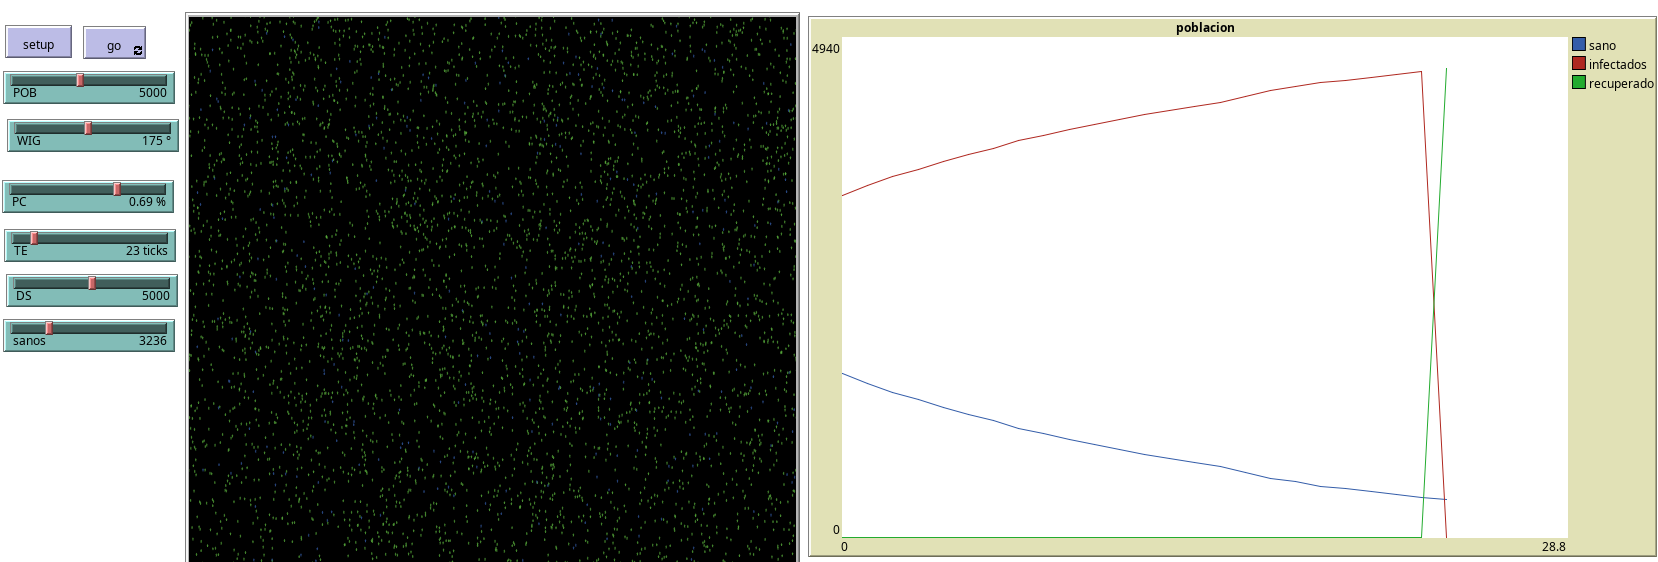
\includegraphics[scale = 0.30]{images/30-50.png}}\\
        en esta ocaciones tenemos $POB=50\%$, $WIG=175$°, $PC=69\%$, $TE=23ticks$, $sanos=30\%$.\\
        
        \textbf{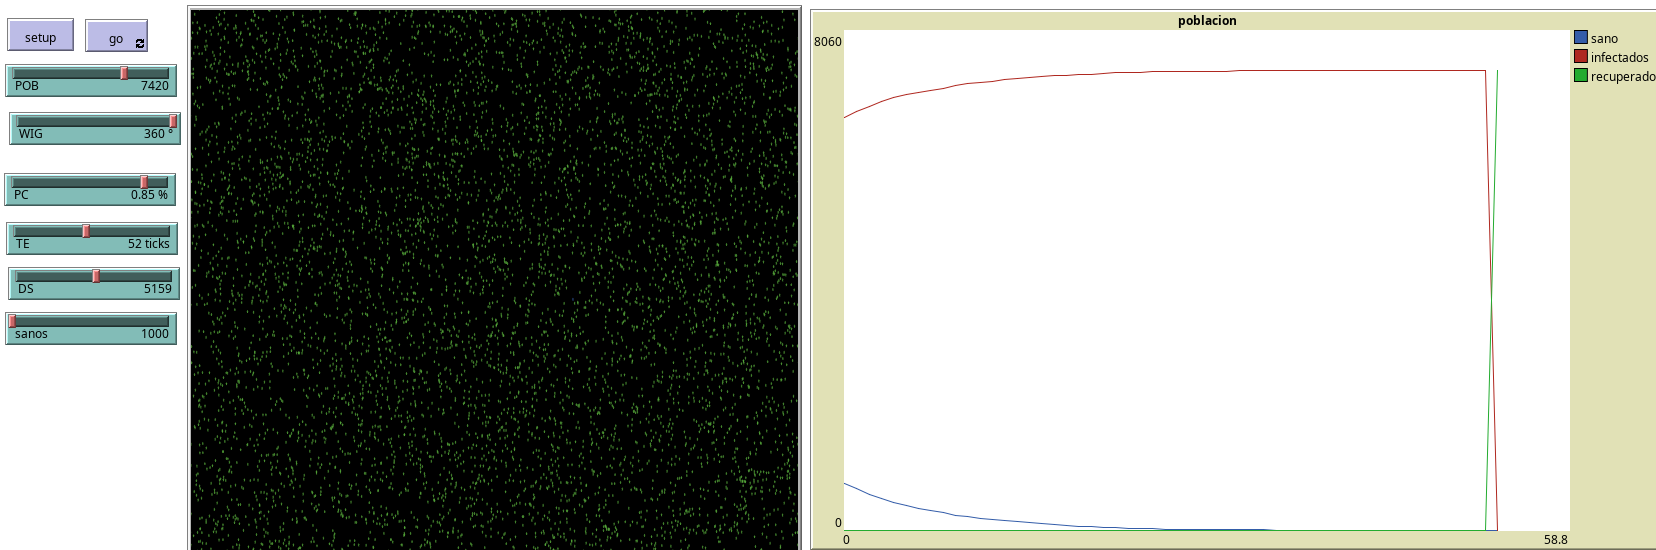
\includegraphics[scale = 0.30]{images/31-50-50.png}}\\
        en esta ocaciones tenemos $POB=70\%$, $WIG=360$°, $PC=86\%$, $TE=50ticks$, $sanos=10\%$.\\
    

        \textbf{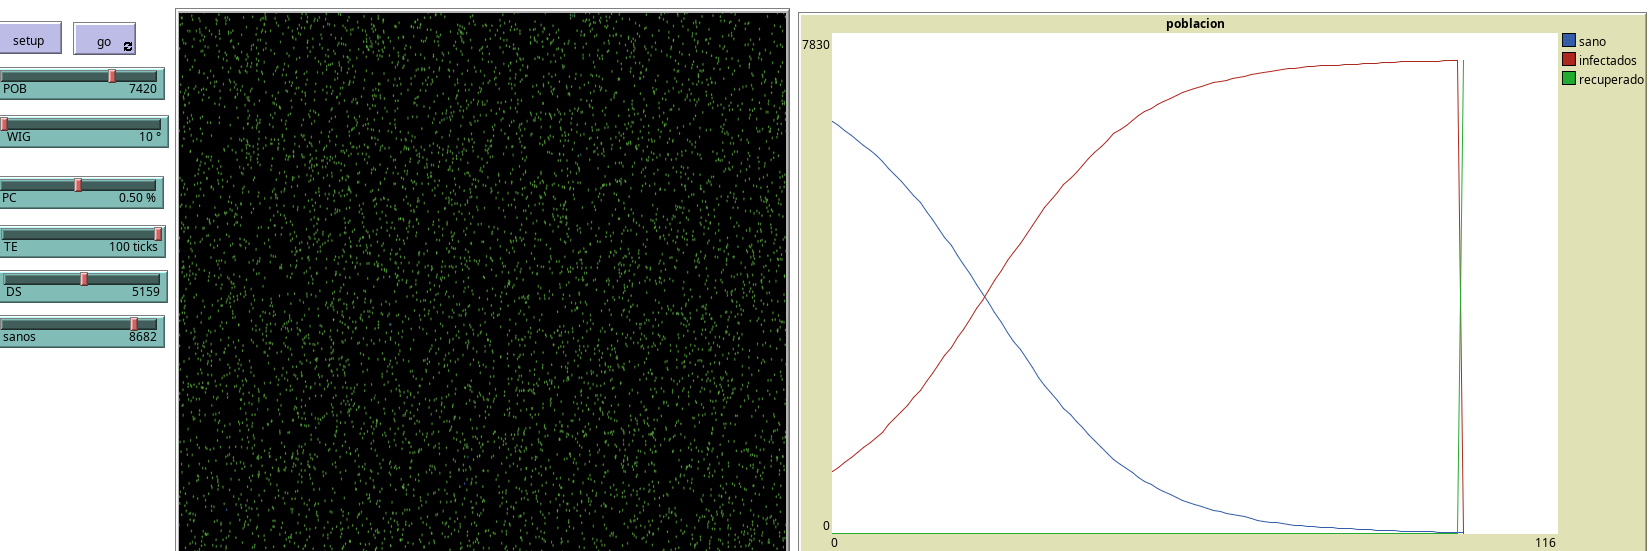
\includegraphics[scale = 0.30]{images/32-50.png}}\\
        en esta ocaciones tenemos $POB=70\%$, $WIG=10$°, $PC=50\%$, $TE=100ticks$, $sanos=80\%$.\\

        
        Con $DS=75\%$:\\

        \textbf{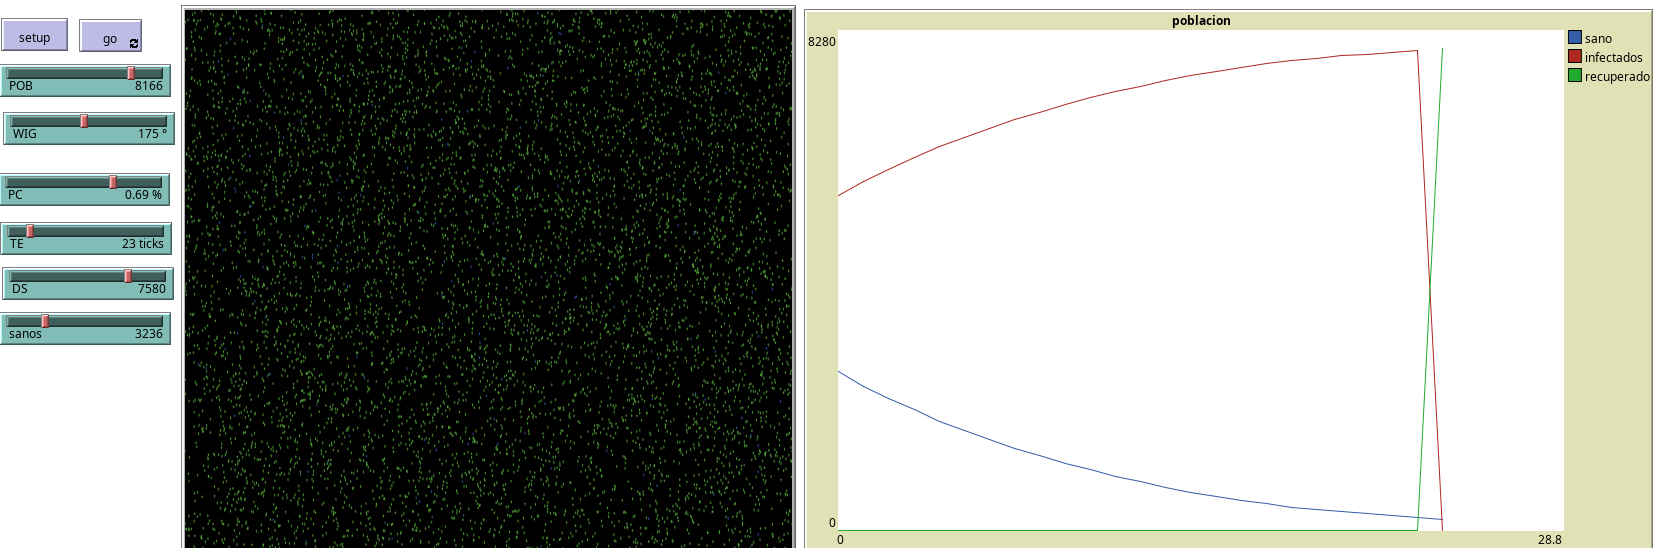
\includegraphics[scale = 0.30]{images/30-75.png}}\\
        en esta ocaciones tenemos $POB=50\%$, $WIG=175$°, $PC=69\%$, $TE=23ticks$, $sanos=30\%$.\\
        
        \textbf{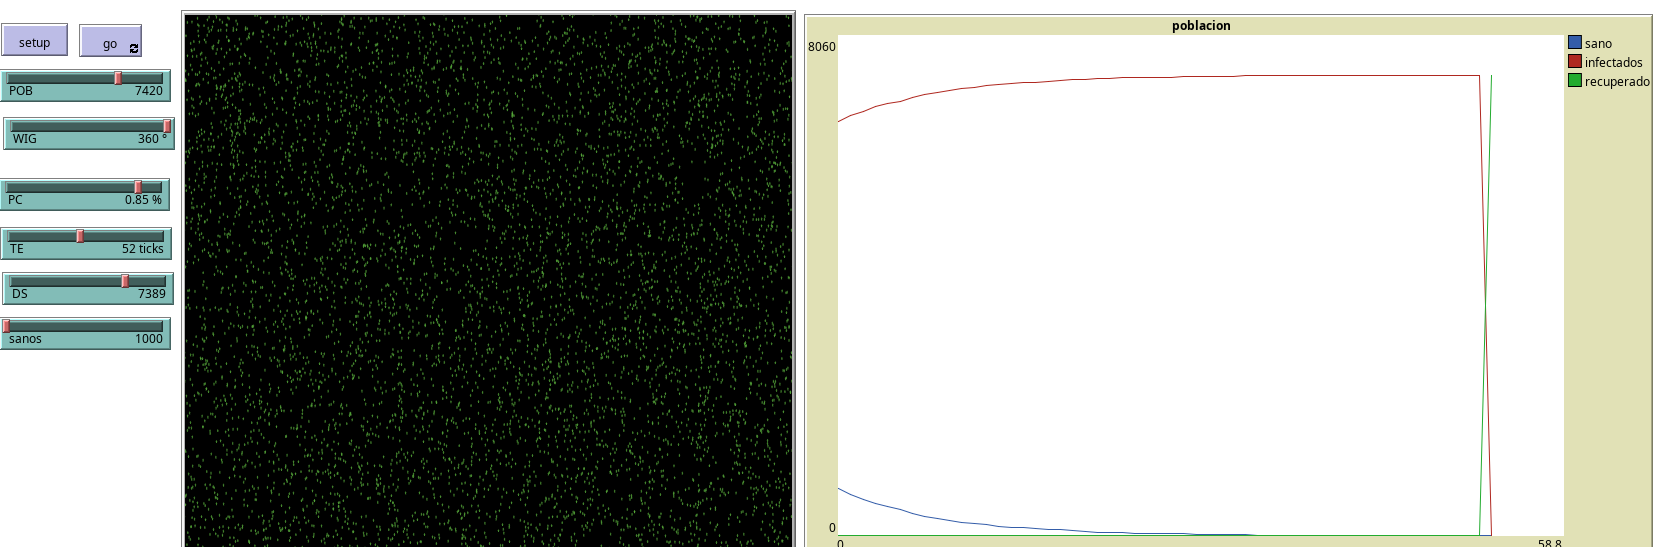
\includegraphics[scale = 0.30]{images/31-50.png}}\\
        en esta ocaciones tenemos $POB=70\%$, $WIG=360$°, $PC=86\%$, $TE=50ticks$, $sanos=10\%$.\\
    

        \textbf{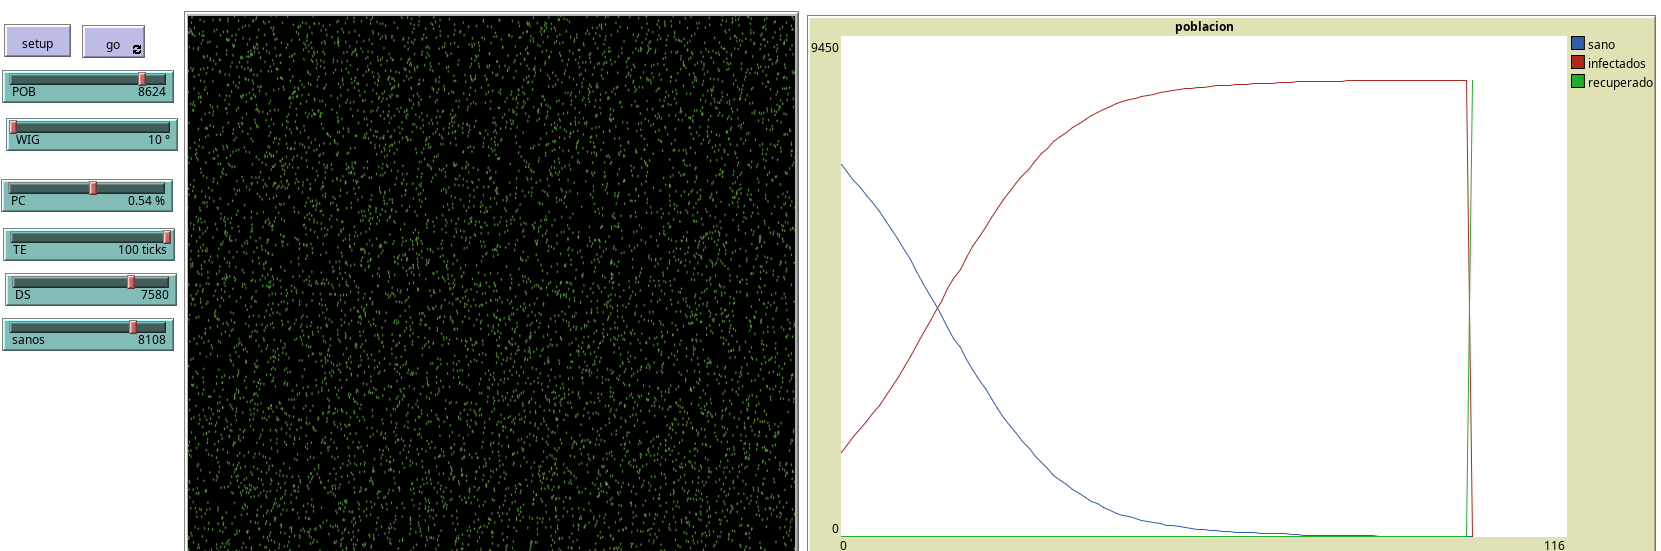
\includegraphics[scale = 0.30]{images/32-75.png}}\\
        en esta ocaciones tenemos $POB=30\%$, $WIG=10$°, $PC=50\%$, $TE=100ticks$, $sanos=80\%$.\\


\end{enumerate}
    Reporte las graficas.\\
    Con $DS=25\%$:\\

    \textbf{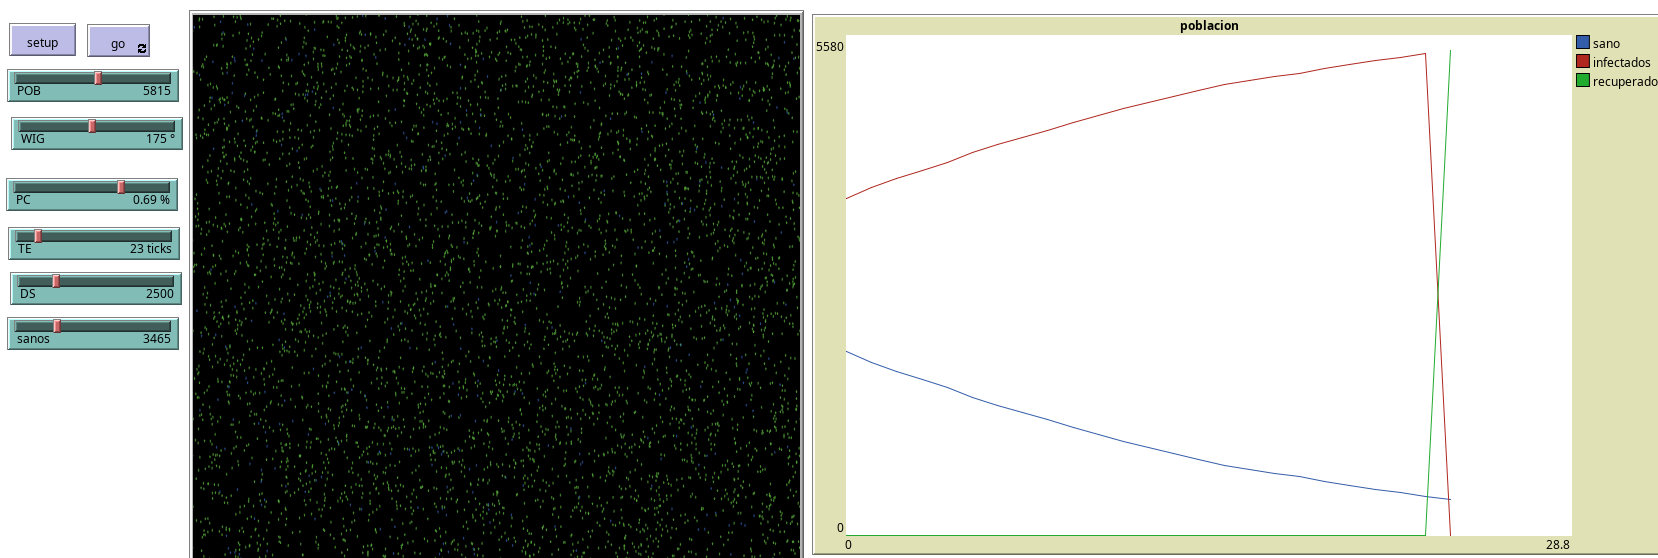
\includegraphics[scale = 0.30]{images/30-25.png}}\\
    en esta ocaciones tenemos $POB=50\%$, $WIG=175$°, $PC=69\%$, $TE=23ticks$, $sanos=30\%$.\\


    \textbf{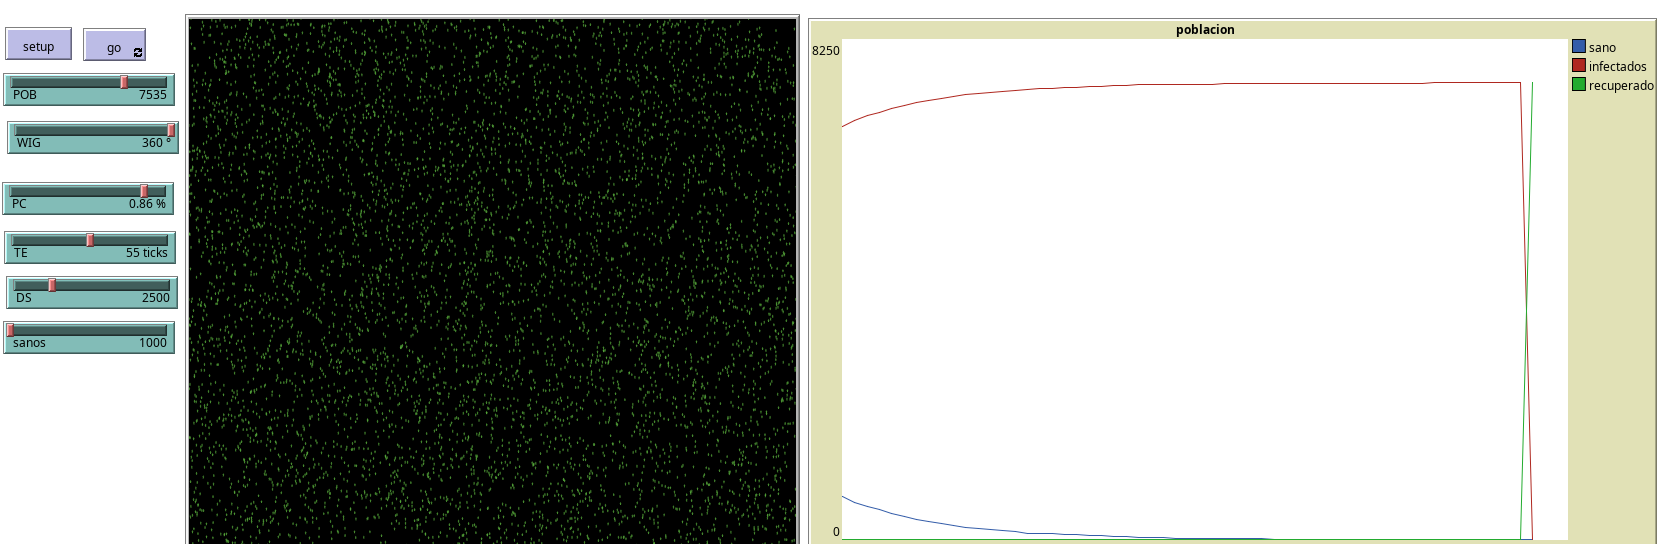
\includegraphics[scale = 0.30]{images/31-25.png}}\\
    en esta ocaciones tenemos $POB=70\%$, $WIG=360$°, $PC=86\%$, $TE=50ticks$, $sanos=10\%$.\\
    


    \textbf{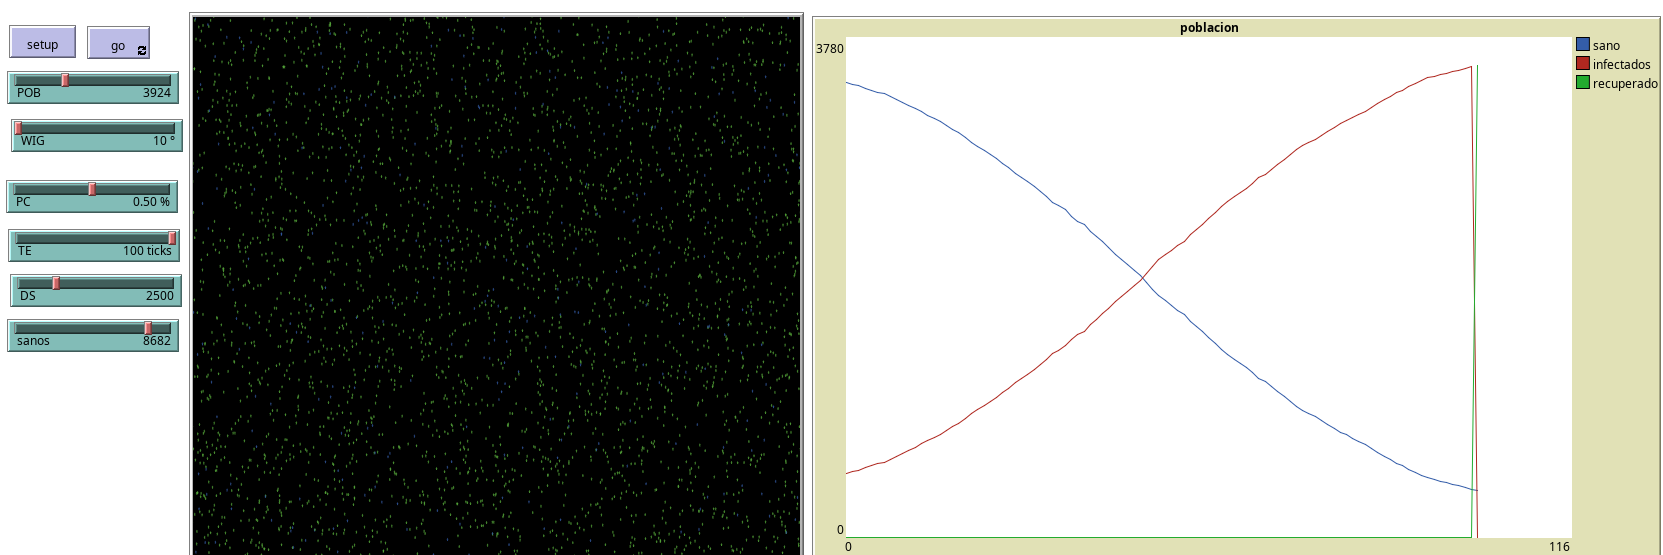
\includegraphics[scale = 0.30]{images/32-25.png}}\\
    en esta ocaciones tenemos $POB=30\%$, $WIG=10$°, $PC=50\%$, $TE=100ticks$, $sanos=80\%$.\\




    \item La curva de infectados alcanza un número máximo de infectados (pico) en un tiempo especifico $t*$, que llamaremos Emax.
    Al variar el paámetro distanciamiento social este valor maximo podría cambiar, para realizar esto, realice la grafica $DS$ vs $Emax$.
    \begin{enumerate}
        \item Explique el comportamiento de la gráfica
        \item Realice la grafica $DS$ vs $t*$, explique el comportamiento.
        \item \textbf{¿Aplicar este tipo de estrategia de contención (distanciamiento social) ayuda a aplanar la curva?}
    \end{enumerate}

    \item \textbf{Conclusión.} Después de sus análisis: 
    \begin{enumerate}
        \item \textbf{¿Qué podría decir del alcance del modelo, funciona para describir, explicar, pronosticar?}
        A mi parecer si funciona aunque en el apartado de distanciamiento social, yo siento que como lo comentamos y vimos en una clase, el aplicar lugar como tipo "refugio" que en la vida real seria estar encerrados en nuestra vivienda, 
        podria funcionar para obtener unos resultados más certeros, pero para su estudio, este modelo con este tipo de funcionamiento no lo veo erroneo, al contrario, a mi forma de analizar y ver como se comportaba el modelo, siento que si es una muy
        buena  aproximación a la realidad a como se vivió con el reciente COVID, es muy interesante, nunca habia oido de este tipo de modelo y me llamó muchisimo la atención del como se comporta en diversas circunstancias.
        \item \textbf{¿Qué posibles extenciones podría proponer?}
        Como lo comente anteriormente podemos agregar en el mundo, apartados como localidades donde los agentes permanezcan un determinado tiempo y asi ver como se comporta y como baja el contagio, tambien podemos agregar la muerte de los agentes si despues de un determinado Tiempo
        no vemos que mejoren, podemos "matarlos" y asi reducir la población y poder tener un contador de los agentes sobrevivientes despues de dertminados ticks, podemos tambien agregar que pueden "curarse" si despues de un tiempo determinado acuden de manera aleatoria en un punto de la simulación, 
        en la que pueden curarse y asi si uno esta curado y se encuentra con alguno que no lo esta, como ya no se puede contagiar, que el que esta en color verde, "oriente" al agente enfermo hacia donde se curo,
        un tanto similar al comportamiento que observamos en la simulacion de las termitas apiladoras pero ahora en lugar de apilar que ese se el punto de cura.
    \end{enumerate}

\end{enumerate}


\end{document}